\documentclass[12pt, a4paper]{article}

\nonstopmode
\usepackage{algorithm}
% \usepackage{algcompatible}
\usepackage{bm}
\usepackage{bbm}
\usepackage{algpseudocode}
\usepackage{amsmath} % flere matematikkommandoer
\usepackage{amssymb} % flere matematikkommandoer
\usepackage{arydshln}
\usepackage[utf8]{inputenc} % æøå
\usepackage[T1]{fontenc} % mere æøå
\usepackage{verbatim} % så man kan skrive ren tekst
\usepackage[all]{xy} % den sidste (avancerede) formel i dokumentet
\usepackage[margin=1in]{geometry}  % set the margins to 1in on all sides
\usepackage{graphicx}              % to include figures
\usepackage{amsfonts}              % for blackboard bold, etc
\usepackage{amsthm}                % better theorem environments
\usepackage{graphicx}
\usepackage{caption}
\usepackage{bm}
\usepackage{pgf}
\usepackage{fancyhdr}
\usepackage{hyperref}
\usepackage{stmaryrd}
\usepackage{mathtools}
\usepackage{multirow}
\usepackage{listings}
\usepackage{subcaption}
\usepackage[inline]{enumitem}
\usepackage[round]{natbib}
\usepackage{breqn}
\usepackage{tikz}
\usetikzlibrary{arrows,automata,fit,positioning, shapes, calc, fadings}

% various theorems, numbered by section

\newtheorem{thm}{Theorem}[section]
\newtheorem{lem}[thm]{Lemma}
\newtheorem{prop}[thm]{Proposition}
\newtheorem{cor}[thm]{Corollary}
\newtheorem{conj}[thm]{Conjecture}

\DeclareMathOperator{\id}{id}
\DeclareMathOperator*{\argmin}{argmin}
\DeclareMathOperator*{\argmax}{argmax}

\newcommand{\nn}{\mathcal{N}}
\newcommand{\uu}{\mathcal{U}}
\newcommand{\bb}{\mathcal{B}}
\newcommand{\ee}{\mathrm{e}}
\newcommand{\rd}[1]{\mathrm{#1}}
\newcommand{\bd}[1]{\mathbf{#1}}  % for bolding symbols
\newcommand{\RR}{\mathbb{R}}      % for Real numbers
\newcommand{\ZZ}{\mathbb{Z}}      % for Integers
\newcommand{\PP}{\mathbb{P}}      % for Prob
\newcommand{\EE}{\mathbb{E}}      % for Expectation
\newcommand{\II}{\mathbbm{1}}      % for Indicator fun
\newcommand{\NN}{\mathbb{N}}      % for Prob
\newcommand{\col}[1]{\left[\begin{matrix} #1 \end{matrix} \right]}
\newcommand{\eqsys}[2]{ \left[\!\!
    \begin{array}{#1} #2
    \end{array}
    \!\!\right]}
\newcommand{\comb}[2]{\binom{#1^2 + #2^2}{#1+#2}}
\newcommand{\sint}[1]{\shortintertext{#1}}
\newcommand{\CTL}[1]{\:\textrm{#1}\:}
\newcommand{\sat}{\:\:\textrm{\textbf{sat}}\:\:}
\newcommand{\pr}{\textrm{Pr}}
\newcommand{\grw}{m_{\mathcal{H}}}
\newcommand{\dvc}{d_{VC}}
\newtheorem{theorem}{Theorem}[section]
\newtheorem{lemma}{Lemma}[theorem]
\newtheorem{Lemma}{Lemma}[section]
\newtheorem{corollary}{Corollary}[theorem]
\newcommand{\lstbg}[3][0pt]{{\fboxsep#1\colorbox{#2}{\strut #3}}}
\newcommand{\kl}{\textrm{kl}}
\newcommand{\KL}{\textrm{KL}}
\newcommand{\hyp}{\mathcal{H}}
\lstdefinelanguage{diff}{
  basicstyle=\ttfamily\scriptsize,
  morecomment=[f][\lstbg{red!20}]-,
  morecomment=[f][\lstbg{green!20}]+,
  morecomment=[f][\textit]{@@},
  %morecomment=[f][\textit]{---},
  %morecomment=[f][\textit]{+++},
}

\newenvironment{gamedef}
{%
 \par\medskip\noindent    
 \textbf{Game Defintion:} \\ % HEADLINE
 \noindent For $t = 1,2,...$:
    \begin{enumerate}[leftmargin=3em,labelsep=1em,beginpenalty=10000]
    \setlength{\itemsep}{0.2em}
    \setlength{\parskip}{0.5em}
    \setlength{\parsep}{0pt}
}
{%
    \end{enumerate}
}
\definecolor{eclipseBlue}{RGB}{42,0.0,255}
\definecolor{eclipseGreen}{RGB}{63,127,95}
\definecolor{eclipsePurple}{RGB}{127,0,85}

\DeclarePairedDelimiterX{\inp}[2]{\langle}{\rangle}{#1, #2}

\lstset{
  language={haskell},
  basicstyle=\ttfamily, % Global Code Style
  captionpos=b, % Position of the Caption (t for top, b for bottom)
  extendedchars=true, % Allows 256 instead of 128 ASCII characters
  tabsize=2, % number of spaces indented when discovering a tab
  columns=fixed, % make all characters equal width
  keepspaces=true, % does not ignore spaces to fit width, convert tabs to spaces
  showstringspaces=false, % lets spaces in strings appear as real spaces
  breaklines=true, % wrap lines if they don't fit
  frame=trbl, % draw a frame at the top, right, left and bottom of the listing
  frameround=tttt, % make the frame round at all four corners
  framesep=4pt, % quarter circle size of the round corners
  numbers=left, % show line numbers at the left
  numberstyle=\small\ttfamily, % style of the line numbers
  commentstyle=\slshape\bfseries\color{eclipseGreen}, % style of comments
  keywordstyle=\bfseries\color{eclipsePurple}, % style of keywords
  stringstyle=\color{eclipseBlue}, % style of strings
  emphstyle=[1]{\color{eclipseBlue}},
  moredelim=**[is][\color{red}]{@@}{@@}
}
\renewcommand{\thesubsubsection}{\thesection.\alph{subsubsection}}
\begin{document}
\author{Chi Pham\\William Sprent}
\title{PFP Exam Project\\Improving Rasterific}
\maketitle

\section{Introduction}
% Noget om hvad projektet går ud på, måske hovedresultater

\section{Background}
% Noget om generel struktur på raste
% Noget om par monad

\section{Experiments}

% Introducer afsnittet, beskriv overordnet hvilke steder vi har identificeret kunne være mulige at parallelisere. måske en tegning ...

\subsection{Benchmarks}

\subsection{Primitives}
Before rasterization, Rasterific works with three different primitive shapes:
lines, quadratic bezier curves, and cubic bezier curves. Each of these are decomposed
to an internal type representing raster lines:
\begin{lstlisting}[caption={\texttt{EdgeSample} type -- represents a raster line.}]
data EdgeSample = EdgeSample
  { _sampleX     :: {-# UNPACK #-} !Float -- ^ Horizontal position
  , _sampleY     :: {-# UNPACK #-} !Float -- ^ Vertical position
  , _sampleAlpha :: {-# UNPACK #-} !Float -- ^ Alpha
  , _sampleH     :: {-# UNPACK #-} !Float -- ^ Height
  }
\end{lstlisting}
This decomposition follows a divide-and-conquer strategy. For example, decomposing a line
involves repeatedly chopping the line in half until both endpoints are in the same pixel.

This pattern seems ripe for parallelisation, however there are a couple of shortfalls:
\begin{itemize}
\item The size of the canvas severely restricts the length of a primitive -- there is no reason to ever
   have a million pixel line.
 \item The decomposition functions returns the following lazy data structure:
   \begin{lstlisting}
     type Producer a = [a] -> [a]\end{lstlisting}
   presumably save the cost of generating a long list of lists just to concatenate them in the end
    when the \texttt{EdgeSamples} are sorted.
  \end{itemize}
  Nevertheless, we have experimented with parallelising the decomposition of primitives.

\subsubsection{Lines}
The \texttt{Graphics.Rasterific.Line} module has the \texttt{decomposeLine} function with type
signature:
\begin{lstlisting}
decomposeLine :: Line -> Producer EdgeSample\end{lstlisting}
We %TODO: finish sentence
\begin{lstlisting}[caption={Naively splitting work in two parts}]
    go !ax !ay !bx !by n cont
    | n == 0  = runPar $ do
        a' <- spawnP $ go ax ay mx my 100 []
        b' <- spawnP $ go mx my bx by 100 []
        b <- get b'
        a <- get a'
        return $ a ++ b ++ cont
\end{lstlisting}
This approach proves to not generate enough work for each thread even when only a single split
is performed. Figure \ref{fig:line-thread} shows ThreadScope out put for only splitting the
work a single time (per line) on two hardware threads. Even with this course distribution of work
26731 of 34000 end up being garbage collected, and we only manage to use 25\% of the available
resources, and running the parallel code with a single thread gives better performance than with
two.
\begin{figure}[h!]
  \centering
  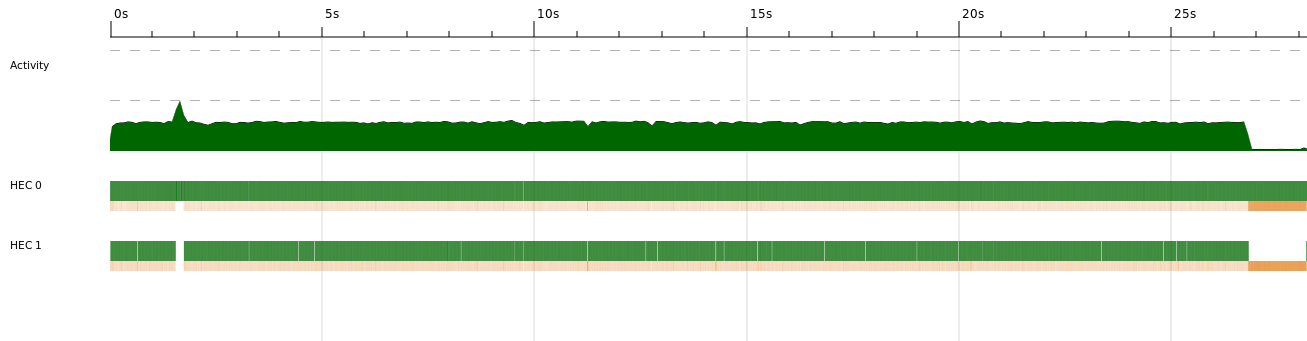
\includegraphics[width=0.85\linewidth]{../threadscope/lines/single-split}
  \caption{ThreadScope output for parallelising line decomposition. Shows the output for the
    \texttt{lines} benchmark.}
  \label{fig:line-thread}
\end{figure}

Inspecting the spark times (Figure \ref{fig:line-thread-sparks}) in ThreadScope confirms that line
decomposition does not produce work enough to justify the hassle --
probably not even to offset any cache locality reduction from working 
on multiple single cores. Most of the converted sparks are completed instantaniously.

\begin{figure}[h!]
  \centering
  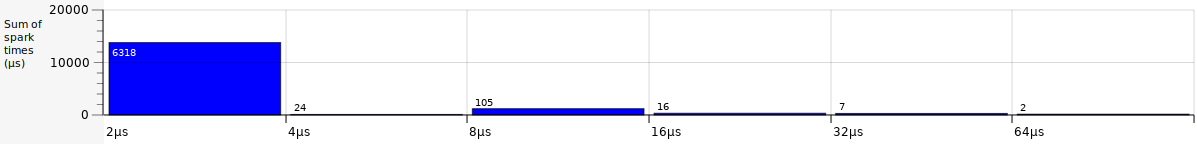
\includegraphics[width=0.85\linewidth]{../threadscope/lines/single-split-spark-times}
  \caption{ThreadScope spark times for Figure \ref{fig:line-thread}}
  \label{fig:line-thread-sparks}
\end{figure}

Investigating further, Figures \ref{fig:single-line-thread} and \ref{fig:single-line-thread-sparks}
show similar results for decomposing a single, \textit{unrealisically} large line where
 we fork at every 10th recursive call. Again we have
 weak utilisation and small spark workloads.

\begin{figure}[h!]
  \centering
  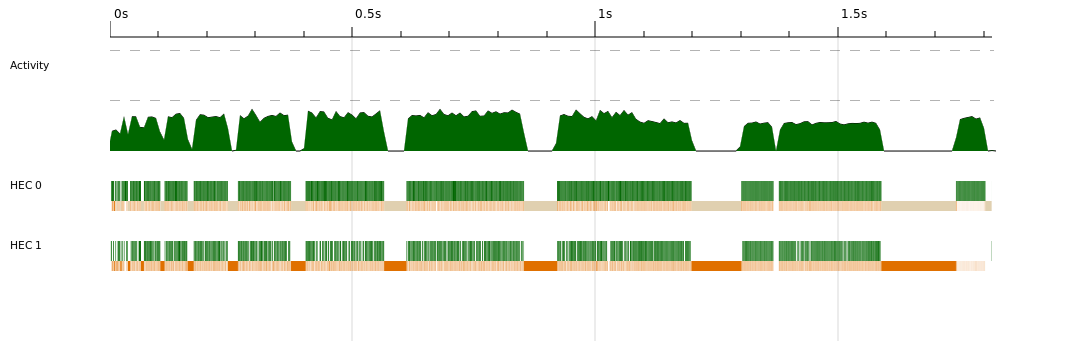
\includegraphics[width=0.85\linewidth]{../threadscope/lines/single-line-every-10}
  \caption{ThreadScope output for running line decomposition on a single line with length
    100000.}
  \label{fig:single-line-thread}
\end{figure}

\begin{figure}[h!]
  \centering
  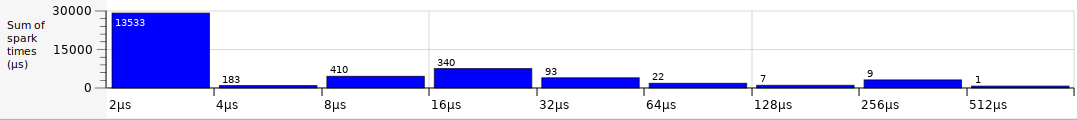
\includegraphics[width=0.85\linewidth]{../threadscope/lines/single-line-every-10-spark-times}
  \caption{ThreadScope output for running line decomposition on a single line with length
    100000.}
  \label{fig:single-line-thread-sparks}
\end{figure}

\subsection{Sorting Edge Samples}

\subsection{Combining Edge Samples}

\subsection{Multiple Decomposition Calls}

\subsection{Multiple FillOrder Calls}

\section{Discussion}

% diskuter resultater
% hvad er scope for parallelisering i det hele taget i rasterific, hvordan kan man udnytte det

\section{Further Work}

\section{Conclusion}



\end{document}
